\documentclass[12pt]{article}
\usepackage{url}
\usepackage[spanish, english]{babel}
\selectlanguage{spanish}
\usepackage[fixlanguage]{babelbib}
\selectbiblanguage{spanish}
\usepackage{url}
\usepackage[utf8]{inputenc}
\usepackage{float}
\usepackage{fullpage}
\usepackage{amsmath}
\usepackage{amssymb}
\usepackage{graphicx}
\usepackage{verbatim} 
\usepackage{caption, subcaption}
\usepackage{tikz}%Generar plots
\usepackage{pgfplots}%Generar plots
\pgfplotsset{compat=1.5}
\usepackage{pgfplotstable,filecontents}
\usepackage{booktabs}
\usepackage{lipsum}

\pgfkeys{/pgf/number format/.cd,fixed,precision=5}

\usepackage[titletoc, title]{appendix}
\addto{\captionsspanish}{\renewcommand*{\appendixname}{Anexo}}

\bibliographystyle{bababbrv}

\title{Segmentación de Piel}
\author{Jorge Bahamonde, Sebastián González\\
\small{\url{jbahamon@ug.uchile.cl}, \url{segonzal@dcc.uchile.cl}}}
\date{}

\begin{document}
\maketitle

\section{Introducción}

% detectar la presencia de un animal es complejo
% perros aun mas porque spn muy diferentes entre razas tamaños texturas del pelaje, etc
% la estrategia de bag of words es una de las tecniacas del reconocimiento de patrones que entrega mejorres resultados
% clasificamos usando lSVM (ibSVM)
% comparamos resultados usando ROC, variando el parametro.

La detección de animales en imágenes es una tarea compleja. La evolución ha llevado a
las criaturas a adaptarce a sus medios, siendo la mímesis con su entorno una de las claves para la supervivencia de las especies.
Los animales domésticos han evolucionado al alero de la humanidad. En tiempos modernos muchos animales viven en entornos urbanos,
y en su rol de mascotas son objetivo de retratos que son subidas a internet por sus dueños.

Presentan un problema adicional. Muchos de estos animales presentan grandes diferencias entres sus razas: tamaño, color, textura, forma, etc.
El estudio de la detección de perros en un conjunto de imágenes es un problema de interés, es un caso representativo de clasificación, para una clase con características
altamente deformables. La ventaja que brinda el estudio sobre imágenes de perros es la alta disponibilidad de imágenesde prueba en internet.
Los perros, siendo una de las mascotas más comunes, marcan una fuerte presencia en los retratos de mascotas en internet.

Se empleó la estrategia Bag of Words, una de las técnicas en el reconocimiento de patrones que arrojan mejores resultados para la clasificación.
Se puso énfasis en el estudio de esta estrategia para el reconocimiento de imágenes de perros. En particular se analizó el desempeño de la clasificación de SVM,
utilizando histogramas de palabras visuales, al variar la razón de costo asociado a los falsos positivos y falsos negativos ($\Theta$).

Se construyó un dataset de 1400 imágenes, de las cuales la mitad contienen imágenes de perros extraidas del dataset Cats and Dogs.
Las restantes imágenes no contienen perros y fueron extraidas aleatoriamente del dataset caltech-101.

\section{Descripción del Trabajo}

Se estudió el desempeño de SVM sobre histogramas de palabras visuales, siguiendo la estrategia Bag of Words.

\subsection{Generación de palabras visuales}

\begin{comment}
A) Generación de palabras visuales mediante clustering: En esta parte, se debe determinar un corpus formado por
5000 imágenes, bajo las cuales se determinarán K palabras visuales. Para obtener el corpus se deben seleccionar
aleatoriamente 5000 imágenes del dataset Caltech-256 (http://www.vision.caltech.edu/Image_Datasets/Caltech256/).
Para cada imagen del corpus se debe calcular descriptores SIFT. Suponiendo que cada imagen genere
aproximadamente 500 descriptores locales, en total tendremos 2.500.000 descriptores. Con el fin de facilitar el
proceso se deben seleccionar aleatoriamente 100.000 descriptores que serán, finalmente, los que determinarán los K
clústers. Luego, las K palabras visuales se obtienen mediante clusterizar el conjunto total de descriptores locales (los
100.000). Una palabra visual estará representada por el centroide de un determinado clúster. Para el proceso de
clustering deben usar la estrategia K-MEANS.
Para obtener los descriptores locales puede usar diferentes libs como:
• VLFeat http://www.vlfeat.org/
• SIFT de OpenCV
• SIFT de Lowe (http://www.cs.ubc.ca/~lowe/keypoints/)
• Affine Covariant Features (http://www.robots.ox.ac.uk/~vgg/research/affine/index.html)
\end{comment}

Se definió un corpus formado por 5000 imágenes extraidas del dataset caltech-256. Para cada imagen se calcularon los descriptores SIFT.
Estos descriptores locales fueron clusterizados utilizando k-means. Los k centroides entregados por este método se utilizaron como
palabras visuales, para la posterior clasificación.

Se generaron palabras visuales para $k = 100, 500, 1000, 1500$.

\subsection{Entrenamiento}

\begin{comment}
B) Entrenamiento usando SVN mediante histogramas Bag of Words: En esta etapa se debe modelar un
clasificador que permita reconocer la ocurrencia de un perro en una imagen. Para este fin, es necesario obtener un
conjunto de entrenamiento. Se recomienda obtener 500 imágenes de perros y 500 imágenes de no-perros. El dataset
Caltech-256 contiene aproximadamente 100 imágenes de perros y miles de imágenes de no perros. Para completar el
dataset de los patrones positivos (imágenes conteniendo un perro) se recomienda obtener las imágenes por Google.
Para facilitar esta tarea, este dataset puede ser compartido entre todos los estudiantes del ramo.
Teniendo el conjunto de entrenamiento, cada imagen se representa como un histograma Bag of Words. Este
histograma representa la distribución de ocurrencias de descriptores locales de la imagen entre los K clústers o
palabras visuales. El histograma debe ser normalizado a la unidad.
La clasificación debe estar basada en la estrategia Support Vector Machine. Para este fin, se recomienda usar
libSVM (http://www.csie.ntu.edu.tw/~cjlin/libsvm/). Deben experimentar con SVM + kernel RBF, los parámetros C y
gamma deberán ser elegidos mediante validación cruzada. LibSVM incluye un pograma en Phyton para obtener los
mejores parámetros.
\end{comment}

Se utilizó la librería libSVM, en particular el script "easy.py" incluido para entrenar cuatro modelos, cada modelo utiliza histogramas de 100, 500, 1000 ó 1500
palabras visuales. Todos los modelos fueron entrenados utilizando 500 imágenes del dataset generado.

\subsection{Clasificación}

Explicar $\Theta$ el ratio de FPR y TPR y bla bla ROC
Esto debe servir para definir el ROC

\subsection{Dataset utilizado}
Se construyó un dataset de 1400 imágenes en total. La mitad de estas imágenes son imágenes de perros extraidas aleatoriamente del dataset Cats and Dogs. 
El resto, 700 imágenes, no contienen perros, y fueron extraidas aleatoriamente del dataset caltech-101.
Se extrajeron 500 imágenes de perros y no-perros para formar parte del set de entrenamiento.
Las 400 imágenes restantes forman el set de prueba.

\section{Resultados obtenidos}

Para evaluar el desempeño del modelo estudiado, se le ultilizó para clasificar imágenes entre dos clases:
Perro y No-Perro. Se contrastaron los resultados obtenidos con la clasificación correcta dada por la distribución en el dataset.

Se definen, en este contexto: 

\begin{itemize}
    \item el \textbf{número de positivos ($P$)} como el número de imágenes en el dataset
        que corresponden a Perros.
    \item el \textbf{número de negativos ($N$)} como el número de imágenes en el dataset
        que no corresponden a Perros.
    \item el \textbf{número de falsos positivos ($FP$)} como el número de
        imágenes en el dataset que el modelo identifica que contiene Perros, pero que no
        están clasificados como tal en el dataset.
    \item el \textbf{número de verdaderos positivos ($TP$)} como el número de
        imágenes en el dataset que el algoritmo identifica que contiene correctamente un Perro.
    \item la \textbf{tasa de verdaderos positivos ($TPR$)} (también llamada
        probabilidad de detección correcta) como $\frac{TP}{P}$;
    \item la \textbf{tasa de falsos positivos ($FPR$)} (o probabilidad de
        detección incorrecta) como $\frac{FP}{N}$.
\end{itemize}

Así, el comportamiento de un modelo de detección como el estudiado puede ser
apreciado al comparar el comportamiento de la $FPR$ versus la $TPR$. La curva
definida por estas dos variables al modificar un tercer parámetro se denomina curva
ROC (del inglés \emph{receiver operating characteristic}). Esta curva muestra
cuán apropiado puede ser un modelo o algoritmo para ciertas aplicaciones, ya que
el costo de un falso positivo versus un verdadero positivo varía dependiendo del
contexto.

\begin{figure}[h]
    \centering
   % \includegraphics{digit}

\begin{tikzpicture}
\begin{axis}[
        title={Curva ROC},
	xlabel={False Positive Rate},
	ylabel={True Positive Rate},
	grid=major,
%	legend entries={$0.01$ , $0.1$,$0.5$},
%	legend style={at={(0,1)},anchor=north west},
]
\addplot table [scatter,x={FPR}, y={TPR}]{results100-ROC.csv};
\addplot table [scatter,x={FPR}, y={TPR}]{results500-ROC.csv};
\addplot table [scatter,x={FPR}, y={TPR}]{results1000-ROC.csv};
\addplot table [scatter,x={FPR}, y={TPR}]{results1500-ROC.csv};
\end{axis}
\end{tikzpicture}
    \caption{Curva ROC obtenida al variar el parámetro umbral $\Theta \in \{ 0.1,0.5,...,0.9,0.91,...0,99\}$.}
\end{figure}

\begin{figure}[H]
    \centering
    \subcaptionbox{No-Perro clasificado como Perro.}
{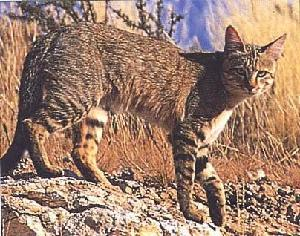
\includegraphics[scale=0.4]{../no-dogs/eval/96.jpg}}
    \subcaptionbox{Perro clasificado como No-Perro.}
{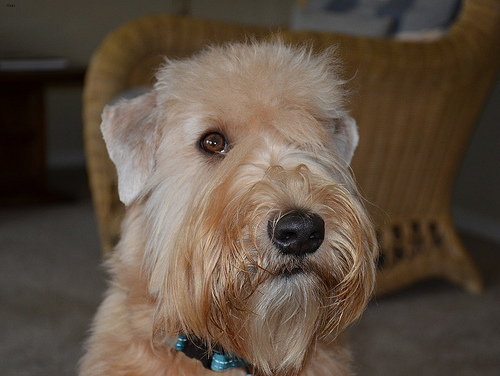
\includegraphics[scale=0.3]{../dogs/eval/3.jpg}}
    \caption{Errores de clasificación.}
\end{figure}

Antes de seguir tengo que arreglar el ROC.


\section{Conclusiones}

\selectlanguage{spanish}
\selectbiblanguage{spanish}

\bibliography{./informe}

\begin{appendices}

\section{Tasas de falsos positivos y verdaderos positivos obtenidas}

\begingroup
\centering
\pgfplotstabletypeset[col sep=tab,
%     columns={theta,FPR,TPR},
     display columns/0/.style={column name=$\Theta$},
     display columns/1/.style={column name=\emph{FalsePositiveRate}},
     display columns/2/.style={column name=\emph{TruePositiveRate}},
     every head row/.style={before row=\toprule,after row=\midrule},
     every last row/.style={after row=\bottomrule},
    ]{results100-ROC.csv}
\captionof{figure}{Tasas de falsos positivos y verdaderos positivos obtenidas.}\label{fig:f}
\endgroup


\end{appendices}


\end{document} 
